\documentclass[11pt]{article}
\usepackage[a4paper,margin=1in]{geometry}
\usepackage{amsmath,amssymb,amsthm}
\usepackage{tikz}
\usepackage{booktabs}
\usepackage{xcolor}
\usepackage[hidelinks]{hyperref}
\hypersetup{pdftitle={Boomerangs in Polya's orchard},pdfauthor={Vamshi Jandhyala}}
\setlength{\parskip}{0.4em}
\setlength{\parindent}{0pt}

\newtheorem{theorem}{Theorem}
\newtheorem{lemma}[theorem]{Lemma}

\definecolor{inkblue}{RGB}{40,76,105}
\definecolor{rust}{RGB}{173,80,45}

\title{Boomerangs in P\'olya's orchard: \\ how far a circular arc can see}
\author{Vamshi Jandhyala}
\date{}

\begin{document}
\maketitle
\vspace{-2em}

\begin{abstract}
Place an open disc of radius $r$ at every nonzero point of the integer lattice. A straight ray from the origin is
blocked within distance about $1/r$; this is P\'olya's orchard problem. Joseph O'Rourke asked on MathOverflow how far
a circular arc from the origin can see, calling the answer $B(r)$. We prove that
\[
\frac4r-10<B(r)\le\frac{28}{r^2}\qquad(0<r\le\tfrac1{10}),
\]
the lower bound holding for all $r\le\frac13$. The lower bound comes from an arc that threads the corridor between
two columns of trees; the upper bound combines Minkowski's theorem for nearly straight arcs, a corridor lemma for
lattice lines of every slope, and the spacing of Farey directions. Exact computations certify arcs reaching
$152.0$ at $r=\frac1{20}$, and the true order of growth, somewhere between $1/r$ and $1/r^2$, remains open. The
inequalities behind both bounds are checked in the Lean proof assistant.
\end{abstract}

\section{The question}

Trees of radius $r$ stand at every lattice point except the origin, where you stand. Looking along a straight line you
can see past a distance $R$ only if $r<1/\sqrt{R^2+1}$, so roughly to distance $1/r$; this is P\'olya's orchard
problem in the sharp form of Allen~\cite{Allen}. O'Rourke~\cite{MO} asked what happens if sight may follow any
circular arc from the origin. Write the \emph{reach} of an arc for the largest distance from the origin it attains
before it first enters a disc, and $B(r)$ for the supremum of the reach over all arcs. An arc of radius $a$ can never
reach beyond $2a$, and a straight line is blocked near $1/r$, so $B(r)$ is finite. The question has had no
answer since 2015. O'Rourke suggested that the best arcs might straddle the discs on the axes.

Before reading on, consider the strip $0<x<1$ between the first two columns of trees. How far could an arc that stays
in that strip get?

\section{The lower bound}

The strip idea works. An arc that starts at the origin almost vertically, bends towards the column $x=1$ and back,
and stays between $x=r$ and $x=1-r$ while it passes the trees, sees about four times as far as any straight line
(Figure~\ref{fig:corridor}).

\begin{theorem}\label{thm:lower}
For $0<r\le\frac13$, $B(r)>\dfrac4r-10$.
\end{theorem}

\begin{proof}
Let the arc leave the origin at angle $\alpha$ to the right of the $y$-axis, turning left, on the circle of radius $a$
with centre $(-a\cos\alpha,\,a\sin\alpha)$; its right branch is $x(y)=-a\cos\alpha+\sqrt{a^2-(y-a\sin\alpha)^2}$. Choose
$a(1-\cos\alpha)=1-r$, so that the widest point of the arc, at height $a\sin\alpha$, is at $x=1-r$. In terms of
$t=\tan(\alpha/2)$ this means $a=(1-r)(1+t^2)/(2t^2)$ and $a\sin\alpha=(1-r)/t$.

\emph{The start.} The arc must be at $x\ge r$ by the time it reaches height $1-r$, to pass the tree at $(0,1)$.
With $A=(1-r)^2$ and $K=1-3r+3r^2$, squaring turns the condition $x(1-r)\ge r$ into
\[
a^2-(1-r-a\sin\alpha)^2-(r+a\cos\alpha)^2=-\frac{Kt^2-2At+r(1-r)}{t^2}\ \ge0,
\]
which holds at the smaller root $t_0=r(1-r)/\bigl(A+\sqrt{A^2-Kr(1-r)}\bigr)$ of the quadratic.

\emph{The passage.} While $0\le y\le1-r$ the arc lies in the square $[0,1-r]^2$, every point of which is at distance
at least $r$ from each nonzero lattice point. For heights with $|y-a\sin\alpha|\le a\sin\alpha-(1-r)$ the arc satisfies
$x(1-r)\le x(y)\le1-r$, so $r\le x\le1-r$, and every such point is at distance at least $r$ from every lattice point.
So the arc enters no disc before height $2a\sin\alpha-(1-r)$, and its reach is at least
\[
\frac{2(1-r)}{t_0}-(1-r)=\frac{2\bigl(A+\sqrt{A^2-Kr(1-r)}\bigr)}{r}-(1-r).
\]
\emph{The estimate.} With $X=Kr(1-r)$ and $\sqrt{A^2-X}\ge A-X/(2A)-X^2/(2A^3)$, this is at least
\[
\frac4r-10+r\Bigl(7-\frac r{1-r}-\frac{K^2}{(1-r)^4}\Bigr),
\]
and the bracket is positive for $r\le\frac13$ because $K\le1$, $(1-r)^4\ge\frac{16}{81}$ and $r/(1-r)\le\frac12$.
\end{proof}

\begin{figure}[ht]
\centering
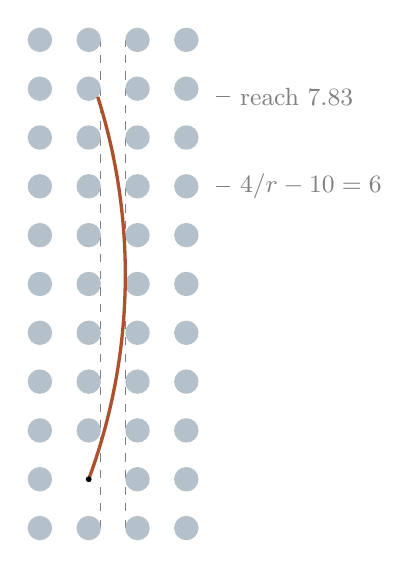
\begin{tikzpicture}[scale=0.62]
  \draw[gray, dashed] (0.25,-1) -- (0.25,9); \draw[gray, dashed] (0.75,-1) -- (0.75,9);
  \fill[inkblue!35] (-1,-1) circle (0.2500);
  \fill[inkblue!35] (-1,0) circle (0.2500);
  \fill[inkblue!35] (-1,1) circle (0.2500);
  \fill[inkblue!35] (-1,2) circle (0.2500);
  \fill[inkblue!35] (-1,3) circle (0.2500);
  \fill[inkblue!35] (-1,4) circle (0.2500);
  \fill[inkblue!35] (-1,5) circle (0.2500);
  \fill[inkblue!35] (-1,6) circle (0.2500);
  \fill[inkblue!35] (-1,7) circle (0.2500);
  \fill[inkblue!35] (-1,8) circle (0.2500);
  \fill[inkblue!35] (-1,9) circle (0.2500);
  \fill[inkblue!35] (0,-1) circle (0.2500);
  \fill[inkblue!35] (0,1) circle (0.2500);
  \fill[inkblue!35] (0,2) circle (0.2500);
  \fill[inkblue!35] (0,3) circle (0.2500);
  \fill[inkblue!35] (0,4) circle (0.2500);
  \fill[inkblue!35] (0,5) circle (0.2500);
  \fill[inkblue!35] (0,6) circle (0.2500);
  \fill[inkblue!35] (0,7) circle (0.2500);
  \fill[inkblue!35] (0,8) circle (0.2500);
  \fill[inkblue!35] (0,9) circle (0.2500);
  \fill[inkblue!35] (1,-1) circle (0.2500);
  \fill[inkblue!35] (1,0) circle (0.2500);
  \fill[inkblue!35] (1,1) circle (0.2500);
  \fill[inkblue!35] (1,2) circle (0.2500);
  \fill[inkblue!35] (1,3) circle (0.2500);
  \fill[inkblue!35] (1,4) circle (0.2500);
  \fill[inkblue!35] (1,5) circle (0.2500);
  \fill[inkblue!35] (1,6) circle (0.2500);
  \fill[inkblue!35] (1,7) circle (0.2500);
  \fill[inkblue!35] (1,8) circle (0.2500);
  \fill[inkblue!35] (1,9) circle (0.2500);
  \fill[inkblue!35] (2,-1) circle (0.2500);
  \fill[inkblue!35] (2,0) circle (0.2500);
  \fill[inkblue!35] (2,1) circle (0.2500);
  \fill[inkblue!35] (2,2) circle (0.2500);
  \fill[inkblue!35] (2,3) circle (0.2500);
  \fill[inkblue!35] (2,4) circle (0.2500);
  \fill[inkblue!35] (2,5) circle (0.2500);
  \fill[inkblue!35] (2,6) circle (0.2500);
  \fill[inkblue!35] (2,7) circle (0.2500);
  \fill[inkblue!35] (2,8) circle (0.2500);
  \fill[inkblue!35] (2,9) circle (0.2500);
  \draw[rust, line width=1.2pt] (0.0000,0.0000) -- (0.0172,0.0468) -- (0.0342,0.0937) -- (0.0511,0.1406) -- (0.0677,0.1876) -- (0.0841,0.2347) -- (0.1004,0.2819) -- (0.1164,0.3291) -- (0.1323,0.3764) -- (0.1480,0.4237) -- (0.1634,0.4711) -- (0.1787,0.5186) -- (0.1938,0.5662) -- (0.2086,0.6138) -- (0.2233,0.6614) -- (0.2378,0.7092) -- (0.2521,0.7569) -- (0.2661,0.8048) -- (0.2800,0.8527) -- (0.2937,0.9006) -- (0.3072,0.9487) -- (0.3205,0.9967) -- (0.3336,1.0448) -- (0.3465,1.0930) -- (0.3592,1.1412) -- (0.3717,1.1895) -- (0.3840,1.2379) -- (0.3961,1.2862) -- (0.4080,1.3347) -- (0.4196,1.3832) -- (0.4311,1.4317) -- (0.4424,1.4803) -- (0.4535,1.5289) -- (0.4644,1.5776) -- (0.4751,1.6263) -- (0.4856,1.6750) -- (0.4959,1.7238) -- (0.5060,1.7727) -- (0.5158,1.8216) -- (0.5255,1.8705) -- (0.5350,1.9194) -- (0.5443,1.9684) -- (0.5533,2.0175) -- (0.5622,2.0666) -- (0.5709,2.1157) -- (0.5793,2.1648) -- (0.5876,2.2140) -- (0.5956,2.2632) -- (0.6035,2.3125) -- (0.6111,2.3618) -- (0.6186,2.4111) -- (0.6258,2.4604) -- (0.6329,2.5098) -- (0.6397,2.5592) -- (0.6463,2.6086) -- (0.6528,2.6581) -- (0.6590,2.7076) -- (0.6650,2.7571) -- (0.6708,2.8066) -- (0.6764,2.8561) -- (0.6818,2.9057) -- (0.6870,2.9553) -- (0.6920,3.0050) -- (0.6968,3.0546) -- (0.7013,3.1043) -- (0.7057,3.1539) -- (0.7099,3.2036) -- (0.7138,3.2533) -- (0.7176,3.3031) -- (0.7211,3.3528) -- (0.7245,3.4026) -- (0.7276,3.4524) -- (0.7306,3.5021) -- (0.7333,3.5519) -- (0.7358,3.6017) -- (0.7381,3.6516) -- (0.7402,3.7014) -- (0.7421,3.7512) -- (0.7438,3.8011) -- (0.7453,3.8509) -- (0.7466,3.9008) -- (0.7477,3.9506) -- (0.7486,4.0005) -- (0.7492,4.0504) -- (0.7497,4.1002) -- (0.7499,4.1501) -- (0.7500,4.2000) -- (0.7498,4.2499) -- (0.7495,4.2997) -- (0.7489,4.3496) -- (0.7481,4.3995) -- (0.7471,4.4493) -- (0.7459,4.4992) -- (0.7445,4.5490) -- (0.7429,4.5989) -- (0.7411,4.6487) -- (0.7391,4.6985) -- (0.7369,4.7484) -- (0.7345,4.7982) -- (0.7318,4.8480) -- (0.7290,4.8978) -- (0.7260,4.9476) -- (0.7227,4.9973) -- (0.7193,5.0471) -- (0.7156,5.0968) -- (0.7117,5.1465) -- (0.7077,5.1962) -- (0.7034,5.2459) -- (0.6989,5.2956) -- (0.6942,5.3452) -- (0.6893,5.3949) -- (0.6842,5.4445) -- (0.6789,5.4941) -- (0.6734,5.5436) -- (0.6677,5.5932) -- (0.6618,5.6427) -- (0.6556,5.6922) -- (0.6493,5.7417) -- (0.6428,5.7911) -- (0.6360,5.8405) -- (0.6291,5.8899) -- (0.6219,5.9393) -- (0.6146,5.9886) -- (0.6070,6.0379) -- (0.5993,6.0872) -- (0.5913,6.1364) -- (0.5832,6.1856) -- (0.5748,6.2347) -- (0.5662,6.2839) -- (0.5574,6.3330) -- (0.5485,6.3820) -- (0.5393,6.4310) -- (0.5299,6.4800) -- (0.5203,6.5290) -- (0.5105,6.5779) -- (0.5005,6.6267) -- (0.4903,6.6756) -- (0.4799,6.7243) -- (0.4693,6.7731) -- (0.4585,6.8218) -- (0.4475,6.8704) -- (0.4363,6.9190) -- (0.4249,6.9675) -- (0.4133,7.0161) -- (0.4015,7.0645) -- (0.3895,7.1129) -- (0.3773,7.1613) -- (0.3649,7.2096) -- (0.3523,7.2578) -- (0.3395,7.3060) -- (0.3265,7.3542) -- (0.3133,7.4023) -- (0.2999,7.4503) -- (0.2863,7.4983) -- (0.2725,7.5462) -- (0.2586,7.5941) -- (0.2444,7.6419) -- (0.2300,7.6896) -- (0.2154,7.7373) -- (0.2006,7.7850) -- (0.1856,7.8325);
  \fill[black] (0,0) circle (0.06);
  \draw[gray] (2.6,7.835) -- (2.9,7.835) node[right, font=\small] {reach $7.83$};
  \draw[gray] (2.6,6.000) -- (2.9,6.000) node[right, font=\small] {$4/r-10=6$};
\end{tikzpicture}

\caption{The corridor arc of Theorem~\ref{thm:lower} at $r=\frac14$, drawn to scale. It leaves the origin almost
vertically, clears the tree at $(0,1)$, and stays between the dashed lines $x=r$ and $x=1-r$, where no disc can
reach it. The proof gives reach at least $7.62$; the arc first touches a disc at distance $7.83$.}
\label{fig:corridor}
\end{figure}

\section{The upper bound}

An arc of radius $a$ that survives an arclength $\ell\le\pi a$ reaches $D=2a\sin\lambda$, $\lambda=\ell/(2a)$. Its
second half turns through an angle $\lambda$, so its directions fill an interval $J$ of length $\lambda$, and it stays
at distance at least $D/2$ from the origin. We bound $\lambda$ in three ranges of $a$.

\emph{Small $a$.} If $a\le2/r^2$ then $D\le2a\le4/r^2$.

\emph{Large $a$.} If $a\ge4/r^3$ the arc is nearly straight. The closed rectangle with half-length $L=3/(2r)$ along
the initial tangent and half-width $2r/3$ across it has area $4$, so by Minkowski's convex body theorem~\cite[Ch.~III]{Cassels}
it contains a lattice point $q\ne0$, which we may take ahead of the origin. Over that length the arc stays within
$a-\sqrt{a^2-L^2}\le0.29\,r$ of the tangent, so it passes within $\frac23r+0.29r<r$ of $q$: $D<3/(2r)+r$. (This is the
idea of Willie Wong's comment on the question.)

\emph{The middle range} needs two lemmas. For a primitive lattice vector $v$ of length $m$, the lattice points lie on
the lines parallel to $v$, which are $1/m$ apart, and are spaced $m$ apart along each line.

\begin{lemma}[corridor lemma]\label{lem:corridor}
Let a piece of an arc of radius $a$, at distance at least $r$ from the origin, turn from the direction of $v$ through an
angle $\varepsilon<\pi/2$ with $\tan\varepsilon<2r/m$. If it avoids every disc, its sideways displacement relative to
$v$ is less than $1/m+2r$. Hence if $a(1-\cos\varepsilon)\ge1/m+2r$, the direction interval $J$ of a surviving arc
cannot contain $[u,u+\varepsilon]$, where $u$ is the direction of $v$.
\end{lemma}

\begin{proof}
In coordinates along and across $v$, the piece is $\varphi\mapsto(\ell_0+a\sin\varphi,\ \tau_0+a(1-\cos\varphi))$ for
$0\le\varphi\le\varepsilon$. If its sideways range covered a whole band $|\tau-k/m|\le r$ around a lattice line,
take $\varphi_1<\varphi_2$ where it enters and leaves the band. Then $a(\cos\varphi_1-\cos\varphi_2)=2r$, and
$\cos(\varepsilon-\varphi_2)\ge\cos(\varepsilon-\varphi_1)$ gives
$a(\sin\varphi_2-\sin\varphi_1)\sin\varepsilon\ge2r\cos\varepsilon$: the piece travels more than $2r\cot\varepsilon>m$
along the line while inside the band. So it passes a lattice point of that line at the same position along the line,
and there it is strictly within $r$ of it; that point is not the origin. A sideways range of at least $1/m+2r$ always
covers a whole band.
\end{proof}

\begin{lemma}[Farey directions]\label{lem:farey}
Let $Q\ge2$. Two primitive vectors of length at most $Q$ that are consecutive in direction make an angle less than
$\pi/Q$.
\end{lemma}

\begin{proof}
If $u,w$ are consecutive, the triangle $0,u,w$ contains no other lattice point: such a point would have length at
most $Q$ and a direction strictly between, or would make $u$ or $w$ imprimitive. By Pick's theorem~\cite{BOOK} the
triangle has area $\frac12$, so $|\det(u,w)|=1$. Then $u+w$ is primitive with direction between them, so $|u+w|>Q$,
hence $|u|+|w|>Q$ and $|u||w|>Q-1$. The angle $\theta$ between them has $\sin\theta=1/(|u||w|)<1/(Q-1)$, and
Jordan's inequality $\sin\theta\ge2\theta/\pi$ gives $\theta<\pi/(2(Q-1))\le\pi/Q$.
\end{proof}

\begin{theorem}\label{thm:upper}
For $0<r\le\frac1{10}$, $B(r)\le\dfrac{28}{r^2}$.
\end{theorem}

\begin{proof}
It remains to treat $2/r^2<a<4/r^3$. Put $Q=\min(ar^2,\sqrt{ar}/2)$, which is at least $2$. For a primitive $v$ of
length $m\le Q$ let $\varepsilon_m=1.01\sqrt{2(1/m+2r)/a}$. Then $\varepsilon_m^2\le0.0123$, and Taylor bounds for
cosine and tangent give $a(1-\cos\varepsilon_m)\ge1/m+2r$ and $\tan\varepsilon_m<2r/m$; the second uses
$m+2rm^2\le\frac32ar^2$, which is where both parts of the definition of $Q$ enter. By Lemma~\ref{lem:corridor}, $J$
contains no interval $[u,u+\varepsilon_m]$, and so none of length $\bar\varepsilon=1.01\sqrt{2(1+2r)/a}\ge\varepsilon_m$
starting at such a direction. By Lemma~\ref{lem:farey} the directions of these $v$ are less than $\pi/Q$ apart, so
$\lambda<\pi/Q+\bar\varepsilon$ and
\[
D\le2a\lambda<\frac{2\pi a}Q+2.02\sqrt{2(1+2r)a}\le\frac{8\pi}{r^2}+\frac2{r^2}<\frac{28}{r^2}.
\]
Together with the other two ranges this proves the theorem.
\end{proof}

The constant is generous. Running the same argument numerically, with the exact Farey gaps and the exact $\varepsilon$
for each $v$ on a fine grid of $a$, gives about $8.6/r^2$ at $r=\frac14$, $6.7/r^2$ at $r=\frac1{10}$ and $6.0/r^2$ at
$r=\frac1{20}$; this evaluation is numerical, not part of the proof.

\section{Computed arcs}

For a fixed radius $a$, all arcs from the origin are rotations of one curve, and each disc forbids an interval of
starting directions that can be computed exactly. Scanning $a$ and polishing the best candidates gives the arcs in
Table~\ref{tab:arcs}. Each is certified afterwards by computing, in $60$-digit arithmetic, where it first enters a
disc; Figure~\ref{fig:best} shows the one for $r=\frac16$. The search can only give lower bounds, and it could miss
narrow optima.

\begin{table}[ht]
\centering
\begin{tabular}{rrrrrrrrr}
\toprule
$1/r$ & 4 & 5 & 6 & 8 & 10 & 12 & 16 & 20 \\
\midrule
$B(r)\ge$ & 9.909 & 13.925 & 18.980 & 31.926 & 43.793 & 65.021 & 111.682 & 151.995 \\
$B\,r^2\ge$ & 0.619 & 0.557 & 0.527 & 0.498 & 0.437 & 0.451 & 0.436 & 0.379 \\
\bottomrule
\end{tabular}
\caption{Certified arcs. For comparison, straight lines reach about $1/r$ and the corridor arc about $4/r$.}
\label{tab:arcs}
\end{table}

\begin{figure}[ht]
\centering
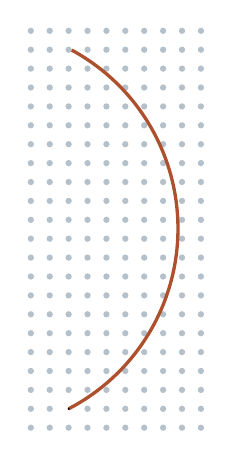
\begin{tikzpicture}[scale=0.24]
  \fill[inkblue!35] (-2,-1) circle (0.1667);
  \fill[inkblue!35] (-2,0) circle (0.1667);
  \fill[inkblue!35] (-2,1) circle (0.1667);
  \fill[inkblue!35] (-2,2) circle (0.1667);
  \fill[inkblue!35] (-2,3) circle (0.1667);
  \fill[inkblue!35] (-2,4) circle (0.1667);
  \fill[inkblue!35] (-2,5) circle (0.1667);
  \fill[inkblue!35] (-2,6) circle (0.1667);
  \fill[inkblue!35] (-2,7) circle (0.1667);
  \fill[inkblue!35] (-2,8) circle (0.1667);
  \fill[inkblue!35] (-2,9) circle (0.1667);
  \fill[inkblue!35] (-2,10) circle (0.1667);
  \fill[inkblue!35] (-2,11) circle (0.1667);
  \fill[inkblue!35] (-2,12) circle (0.1667);
  \fill[inkblue!35] (-2,13) circle (0.1667);
  \fill[inkblue!35] (-2,14) circle (0.1667);
  \fill[inkblue!35] (-2,15) circle (0.1667);
  \fill[inkblue!35] (-2,16) circle (0.1667);
  \fill[inkblue!35] (-2,17) circle (0.1667);
  \fill[inkblue!35] (-2,18) circle (0.1667);
  \fill[inkblue!35] (-2,19) circle (0.1667);
  \fill[inkblue!35] (-2,20) circle (0.1667);
  \fill[inkblue!35] (-1,-1) circle (0.1667);
  \fill[inkblue!35] (-1,0) circle (0.1667);
  \fill[inkblue!35] (-1,1) circle (0.1667);
  \fill[inkblue!35] (-1,2) circle (0.1667);
  \fill[inkblue!35] (-1,3) circle (0.1667);
  \fill[inkblue!35] (-1,4) circle (0.1667);
  \fill[inkblue!35] (-1,5) circle (0.1667);
  \fill[inkblue!35] (-1,6) circle (0.1667);
  \fill[inkblue!35] (-1,7) circle (0.1667);
  \fill[inkblue!35] (-1,8) circle (0.1667);
  \fill[inkblue!35] (-1,9) circle (0.1667);
  \fill[inkblue!35] (-1,10) circle (0.1667);
  \fill[inkblue!35] (-1,11) circle (0.1667);
  \fill[inkblue!35] (-1,12) circle (0.1667);
  \fill[inkblue!35] (-1,13) circle (0.1667);
  \fill[inkblue!35] (-1,14) circle (0.1667);
  \fill[inkblue!35] (-1,15) circle (0.1667);
  \fill[inkblue!35] (-1,16) circle (0.1667);
  \fill[inkblue!35] (-1,17) circle (0.1667);
  \fill[inkblue!35] (-1,18) circle (0.1667);
  \fill[inkblue!35] (-1,19) circle (0.1667);
  \fill[inkblue!35] (-1,20) circle (0.1667);
  \fill[inkblue!35] (0,-1) circle (0.1667);
  \fill[inkblue!35] (0,1) circle (0.1667);
  \fill[inkblue!35] (0,2) circle (0.1667);
  \fill[inkblue!35] (0,3) circle (0.1667);
  \fill[inkblue!35] (0,4) circle (0.1667);
  \fill[inkblue!35] (0,5) circle (0.1667);
  \fill[inkblue!35] (0,6) circle (0.1667);
  \fill[inkblue!35] (0,7) circle (0.1667);
  \fill[inkblue!35] (0,8) circle (0.1667);
  \fill[inkblue!35] (0,9) circle (0.1667);
  \fill[inkblue!35] (0,10) circle (0.1667);
  \fill[inkblue!35] (0,11) circle (0.1667);
  \fill[inkblue!35] (0,12) circle (0.1667);
  \fill[inkblue!35] (0,13) circle (0.1667);
  \fill[inkblue!35] (0,14) circle (0.1667);
  \fill[inkblue!35] (0,15) circle (0.1667);
  \fill[inkblue!35] (0,16) circle (0.1667);
  \fill[inkblue!35] (0,17) circle (0.1667);
  \fill[inkblue!35] (0,18) circle (0.1667);
  \fill[inkblue!35] (0,19) circle (0.1667);
  \fill[inkblue!35] (0,20) circle (0.1667);
  \fill[inkblue!35] (1,-1) circle (0.1667);
  \fill[inkblue!35] (1,0) circle (0.1667);
  \fill[inkblue!35] (1,1) circle (0.1667);
  \fill[inkblue!35] (1,2) circle (0.1667);
  \fill[inkblue!35] (1,3) circle (0.1667);
  \fill[inkblue!35] (1,4) circle (0.1667);
  \fill[inkblue!35] (1,5) circle (0.1667);
  \fill[inkblue!35] (1,6) circle (0.1667);
  \fill[inkblue!35] (1,7) circle (0.1667);
  \fill[inkblue!35] (1,8) circle (0.1667);
  \fill[inkblue!35] (1,9) circle (0.1667);
  \fill[inkblue!35] (1,10) circle (0.1667);
  \fill[inkblue!35] (1,11) circle (0.1667);
  \fill[inkblue!35] (1,12) circle (0.1667);
  \fill[inkblue!35] (1,13) circle (0.1667);
  \fill[inkblue!35] (1,14) circle (0.1667);
  \fill[inkblue!35] (1,15) circle (0.1667);
  \fill[inkblue!35] (1,16) circle (0.1667);
  \fill[inkblue!35] (1,17) circle (0.1667);
  \fill[inkblue!35] (1,18) circle (0.1667);
  \fill[inkblue!35] (1,19) circle (0.1667);
  \fill[inkblue!35] (1,20) circle (0.1667);
  \fill[inkblue!35] (2,-1) circle (0.1667);
  \fill[inkblue!35] (2,0) circle (0.1667);
  \fill[inkblue!35] (2,1) circle (0.1667);
  \fill[inkblue!35] (2,2) circle (0.1667);
  \fill[inkblue!35] (2,3) circle (0.1667);
  \fill[inkblue!35] (2,4) circle (0.1667);
  \fill[inkblue!35] (2,5) circle (0.1667);
  \fill[inkblue!35] (2,6) circle (0.1667);
  \fill[inkblue!35] (2,7) circle (0.1667);
  \fill[inkblue!35] (2,8) circle (0.1667);
  \fill[inkblue!35] (2,9) circle (0.1667);
  \fill[inkblue!35] (2,10) circle (0.1667);
  \fill[inkblue!35] (2,11) circle (0.1667);
  \fill[inkblue!35] (2,12) circle (0.1667);
  \fill[inkblue!35] (2,13) circle (0.1667);
  \fill[inkblue!35] (2,14) circle (0.1667);
  \fill[inkblue!35] (2,15) circle (0.1667);
  \fill[inkblue!35] (2,16) circle (0.1667);
  \fill[inkblue!35] (2,17) circle (0.1667);
  \fill[inkblue!35] (2,18) circle (0.1667);
  \fill[inkblue!35] (2,19) circle (0.1667);
  \fill[inkblue!35] (2,20) circle (0.1667);
  \fill[inkblue!35] (3,-1) circle (0.1667);
  \fill[inkblue!35] (3,0) circle (0.1667);
  \fill[inkblue!35] (3,1) circle (0.1667);
  \fill[inkblue!35] (3,2) circle (0.1667);
  \fill[inkblue!35] (3,3) circle (0.1667);
  \fill[inkblue!35] (3,4) circle (0.1667);
  \fill[inkblue!35] (3,5) circle (0.1667);
  \fill[inkblue!35] (3,6) circle (0.1667);
  \fill[inkblue!35] (3,7) circle (0.1667);
  \fill[inkblue!35] (3,8) circle (0.1667);
  \fill[inkblue!35] (3,9) circle (0.1667);
  \fill[inkblue!35] (3,10) circle (0.1667);
  \fill[inkblue!35] (3,11) circle (0.1667);
  \fill[inkblue!35] (3,12) circle (0.1667);
  \fill[inkblue!35] (3,13) circle (0.1667);
  \fill[inkblue!35] (3,14) circle (0.1667);
  \fill[inkblue!35] (3,15) circle (0.1667);
  \fill[inkblue!35] (3,16) circle (0.1667);
  \fill[inkblue!35] (3,17) circle (0.1667);
  \fill[inkblue!35] (3,18) circle (0.1667);
  \fill[inkblue!35] (3,19) circle (0.1667);
  \fill[inkblue!35] (3,20) circle (0.1667);
  \fill[inkblue!35] (4,-1) circle (0.1667);
  \fill[inkblue!35] (4,0) circle (0.1667);
  \fill[inkblue!35] (4,1) circle (0.1667);
  \fill[inkblue!35] (4,2) circle (0.1667);
  \fill[inkblue!35] (4,3) circle (0.1667);
  \fill[inkblue!35] (4,4) circle (0.1667);
  \fill[inkblue!35] (4,5) circle (0.1667);
  \fill[inkblue!35] (4,6) circle (0.1667);
  \fill[inkblue!35] (4,7) circle (0.1667);
  \fill[inkblue!35] (4,8) circle (0.1667);
  \fill[inkblue!35] (4,9) circle (0.1667);
  \fill[inkblue!35] (4,10) circle (0.1667);
  \fill[inkblue!35] (4,11) circle (0.1667);
  \fill[inkblue!35] (4,12) circle (0.1667);
  \fill[inkblue!35] (4,13) circle (0.1667);
  \fill[inkblue!35] (4,14) circle (0.1667);
  \fill[inkblue!35] (4,15) circle (0.1667);
  \fill[inkblue!35] (4,16) circle (0.1667);
  \fill[inkblue!35] (4,17) circle (0.1667);
  \fill[inkblue!35] (4,18) circle (0.1667);
  \fill[inkblue!35] (4,19) circle (0.1667);
  \fill[inkblue!35] (4,20) circle (0.1667);
  \fill[inkblue!35] (5,-1) circle (0.1667);
  \fill[inkblue!35] (5,0) circle (0.1667);
  \fill[inkblue!35] (5,1) circle (0.1667);
  \fill[inkblue!35] (5,2) circle (0.1667);
  \fill[inkblue!35] (5,3) circle (0.1667);
  \fill[inkblue!35] (5,4) circle (0.1667);
  \fill[inkblue!35] (5,5) circle (0.1667);
  \fill[inkblue!35] (5,6) circle (0.1667);
  \fill[inkblue!35] (5,7) circle (0.1667);
  \fill[inkblue!35] (5,8) circle (0.1667);
  \fill[inkblue!35] (5,9) circle (0.1667);
  \fill[inkblue!35] (5,10) circle (0.1667);
  \fill[inkblue!35] (5,11) circle (0.1667);
  \fill[inkblue!35] (5,12) circle (0.1667);
  \fill[inkblue!35] (5,13) circle (0.1667);
  \fill[inkblue!35] (5,14) circle (0.1667);
  \fill[inkblue!35] (5,15) circle (0.1667);
  \fill[inkblue!35] (5,16) circle (0.1667);
  \fill[inkblue!35] (5,17) circle (0.1667);
  \fill[inkblue!35] (5,18) circle (0.1667);
  \fill[inkblue!35] (5,19) circle (0.1667);
  \fill[inkblue!35] (5,20) circle (0.1667);
  \fill[inkblue!35] (6,-1) circle (0.1667);
  \fill[inkblue!35] (6,0) circle (0.1667);
  \fill[inkblue!35] (6,1) circle (0.1667);
  \fill[inkblue!35] (6,2) circle (0.1667);
  \fill[inkblue!35] (6,3) circle (0.1667);
  \fill[inkblue!35] (6,4) circle (0.1667);
  \fill[inkblue!35] (6,5) circle (0.1667);
  \fill[inkblue!35] (6,6) circle (0.1667);
  \fill[inkblue!35] (6,7) circle (0.1667);
  \fill[inkblue!35] (6,8) circle (0.1667);
  \fill[inkblue!35] (6,9) circle (0.1667);
  \fill[inkblue!35] (6,10) circle (0.1667);
  \fill[inkblue!35] (6,11) circle (0.1667);
  \fill[inkblue!35] (6,12) circle (0.1667);
  \fill[inkblue!35] (6,13) circle (0.1667);
  \fill[inkblue!35] (6,14) circle (0.1667);
  \fill[inkblue!35] (6,15) circle (0.1667);
  \fill[inkblue!35] (6,16) circle (0.1667);
  \fill[inkblue!35] (6,17) circle (0.1667);
  \fill[inkblue!35] (6,18) circle (0.1667);
  \fill[inkblue!35] (6,19) circle (0.1667);
  \fill[inkblue!35] (6,20) circle (0.1667);
  \fill[inkblue!35] (7,-1) circle (0.1667);
  \fill[inkblue!35] (7,0) circle (0.1667);
  \fill[inkblue!35] (7,1) circle (0.1667);
  \fill[inkblue!35] (7,2) circle (0.1667);
  \fill[inkblue!35] (7,3) circle (0.1667);
  \fill[inkblue!35] (7,4) circle (0.1667);
  \fill[inkblue!35] (7,5) circle (0.1667);
  \fill[inkblue!35] (7,6) circle (0.1667);
  \fill[inkblue!35] (7,7) circle (0.1667);
  \fill[inkblue!35] (7,8) circle (0.1667);
  \fill[inkblue!35] (7,9) circle (0.1667);
  \fill[inkblue!35] (7,10) circle (0.1667);
  \fill[inkblue!35] (7,11) circle (0.1667);
  \fill[inkblue!35] (7,12) circle (0.1667);
  \fill[inkblue!35] (7,13) circle (0.1667);
  \fill[inkblue!35] (7,14) circle (0.1667);
  \fill[inkblue!35] (7,15) circle (0.1667);
  \fill[inkblue!35] (7,16) circle (0.1667);
  \fill[inkblue!35] (7,17) circle (0.1667);
  \fill[inkblue!35] (7,18) circle (0.1667);
  \fill[inkblue!35] (7,19) circle (0.1667);
  \fill[inkblue!35] (7,20) circle (0.1667);
  \draw[rust, line width=1.2pt] (-0.0000,0.0000) -- (0.1285,0.0680) -- (0.2561,0.1377) -- (0.3828,0.2091) -- (0.5084,0.2823) -- (0.6331,0.3571) -- (0.7567,0.4336) -- (0.8793,0.5118) -- (1.0008,0.5916) -- (1.1213,0.6731) -- (1.2406,0.7562) -- (1.3588,0.8409) -- (1.4758,0.9272) -- (1.5916,1.0150) -- (1.7063,1.1045) -- (1.8197,1.1954) -- (1.9319,1.2879) -- (2.0428,1.3819) -- (2.1525,1.4774) -- (2.2608,1.5744) -- (2.3678,1.6728) -- (2.4735,1.7726) -- (2.5778,1.8739) -- (2.6808,1.9766) -- (2.7823,2.0807) -- (2.8824,2.1861) -- (2.9811,2.2929) -- (3.0784,2.4010) -- (3.1741,2.5104) -- (3.2684,2.6211) -- (3.3612,2.7331) -- (3.4524,2.8463) -- (3.5421,2.9607) -- (3.6303,3.0763) -- (3.7168,3.1931) -- (3.8018,3.3111) -- (3.8852,3.4302) -- (3.9670,3.5504) -- (4.0471,3.6718) -- (4.1256,3.7942) -- (4.2024,3.9176) -- (4.2776,4.0421) -- (4.3510,4.1676) -- (4.4228,4.2940) -- (4.4928,4.4215) -- (4.5611,4.5498) -- (4.6276,4.6791) -- (4.6924,4.8092) -- (4.7555,4.9403) -- (4.8167,5.0721) -- (4.8762,5.2048) -- (4.9339,5.3383) -- (4.9897,5.4725) -- (5.0438,5.6075) -- (5.0960,5.7432) -- (5.1463,5.8796) -- (5.1948,6.0167) -- (5.2415,6.1544) -- (5.2863,6.2927) -- (5.3292,6.4316) -- (5.3702,6.5711) -- (5.4093,6.7112) -- (5.4466,6.8517) -- (5.4819,6.9927) -- (5.5153,7.1342) -- (5.5468,7.2762) -- (5.5764,7.4185) -- (5.6041,7.5613) -- (5.6298,7.7044) -- (5.6536,7.8478) -- (5.6754,7.9916) -- (5.6953,8.1356) -- (5.7133,8.2799) -- (5.7292,8.4244) -- (5.7433,8.5691) -- (5.7554,8.7140) -- (5.7655,8.8591) -- (5.7736,9.0042) -- (5.7798,9.1495) -- (5.7840,9.2949) -- (5.7863,9.4402) -- (5.7865,9.5856) -- (5.7849,9.7310) -- (5.7812,9.8764) -- (5.7756,10.0217) -- (5.7680,10.1669) -- (5.7585,10.3119) -- (5.7470,10.4569) -- (5.7335,10.6017) -- (5.7181,10.7462) -- (5.7007,10.8906) -- (5.6814,11.0347) -- (5.6601,11.1785) -- (5.6369,11.3221) -- (5.6117,11.4653) -- (5.5846,11.6081) -- (5.5556,11.7506) -- (5.5246,11.8927) -- (5.4918,12.0343) -- (5.4570,12.1755) -- (5.4203,12.3162) -- (5.3817,12.4563) -- (5.3412,12.5960) -- (5.2988,12.7351) -- (5.2546,12.8736) -- (5.2085,13.0115) -- (5.1605,13.1487) -- (5.1107,13.2853) -- (5.0590,13.4212) -- (5.0055,13.5564) -- (4.9502,13.6909) -- (4.8930,13.8246) -- (4.8341,13.9575) -- (4.7733,14.0896) -- (4.7108,14.2209) -- (4.6465,14.3513) -- (4.5805,14.4808) -- (4.5127,14.6094) -- (4.4431,14.7371) -- (4.3719,14.8639) -- (4.2989,14.9896) -- (4.2243,15.1144) -- (4.1479,15.2381) -- (4.0699,15.3608) -- (3.9903,15.4825) -- (3.9090,15.6030) -- (3.8261,15.7225) -- (3.7415,15.8408) -- (3.6554,15.9579) -- (3.5677,16.0739) -- (3.4785,16.1887) -- (3.3877,16.3022) -- (3.2953,16.4145) -- (3.2015,16.5256) -- (3.1062,16.6354) -- (3.0093,16.7439) -- (2.9111,16.8510) -- (2.8114,16.9569) -- (2.7102,17.0613) -- (2.6077,17.1644) -- (2.5038,17.2661) -- (2.3985,17.3664) -- (2.2918,17.4652) -- (2.1839,17.5626) -- (2.0746,17.6585) -- (1.9641,17.7529) -- (1.8522,17.8459) -- (1.7392,17.9373) -- (1.6249,18.0271) -- (1.5094,18.1155) -- (1.3927,18.2022) -- (1.2748,18.2874) -- (1.1558,18.3709) -- (1.0357,18.4529) -- (0.9145,18.5332) -- (0.7922,18.6118) -- (0.6689,18.6888) -- (0.5445,18.7641) -- (0.4191,18.8378) -- (0.2928,18.9097) -- (0.1655,18.9799);
  \fill[black] (0,0) circle (0.06);
\end{tikzpicture}

\caption{The certified arc for $r=\frac16$, with the trees to scale: radius $10.75$, reach $18.98$.}
\label{fig:best}
\end{figure}

Between $1/r=10$ and $20$ the computed reach grows like $r^{-1.8}$. A heuristic points the other way: a generic arc of
length $\ell$ survives with probability about $e^{-2r\ell}$, and there are polynomially many distinguishable arcs, which
suggests $B(r)\approx c\log(1/r)/r$; the ratio $B\,r/\log(1/r)$ goes from $1.79$ at $r=\frac14$ to $2.54$ at
$r=\frac1{20}$, though not monotonically. We cannot tell these apart.

\section{What is left}

The order of growth of $B(r)$: is it $\log(1/r)/r$, a power of $1/r$ strictly between $1$ and $2$, or $1/r^2$? A proof
that $B(r)\,r\to\infty$, or that $B(r)=o(1/r^2)$, would already be progress. The corridor lemma loses most in the
middle range, where the arc is long but bends through only a small angle.

\paragraph{Verification.} The algebra and clearance facts in the proof of Theorem~\ref{thm:lower} (the root $t_0$,
the starting condition, the corridor $r\le x\le1-r$, the clearance of the box and the strip, and the final estimate),
the corridor lemma, the angle estimate of Lemma~\ref{lem:farey} from $|u|+|w|>Q$, the offset bound for large $a$, the
conditions on $\varepsilon_m$, and the three range estimates are proved in Lean~4 with Mathlib~\cite{mathlib}, using
only the standard axioms. Minkowski's and Pick's theorems are cited, and the circle geometry linking an arc to its
reach and direction interval is elementary. Python scripts check the inequality of Theorem~\ref{thm:lower} for $2000$
values of $r$ and the corridor arc's exact reach for $40$, certify the arcs of Table~\ref{tab:arcs} exactly, evaluate the numerical upper bound and the quoted ratios, and
reject deliberately broken versions; an independent script checks the arcs by dense sampling. Everything is at
\url{https://github.com/jvvk/mathematics/tree/main/boomerangs-polya-orchard}.

\paragraph{Acknowledgements.} Joseph O'Rourke asked the question~\cite{MO}; Willie Wong's comment there contains the
idea used for large radii. Anthropic's Claude (Opus~5.5) was used to derive and check the bounds, run the searches,
write the Lean formalisation and the programs, and draft this text. The author takes responsibility for the content.

\begin{thebibliography}{9}
\bibitem{MO} J.~O'Rourke, Boomerangs in Polya's orchard, MathOverflow question 224015 (2015),
\url{https://mathoverflow.net/q/224015}, accessed 10 October 2026.
\bibitem{Allen} T.~T.~Allen, P\'olya's orchard problem, \emph{Amer. Math. Monthly} \textbf{93} (1986) 98--104,
\href{https://doi.org/10.1080/00029890.1986.11971759}{doi:10.1080/00029890.1986.11971759}.
\bibitem{Cassels} J.~W.~S.~Cassels, \emph{An Introduction to the Geometry of Numbers}, Springer, 1959; Chapter III,
Theorems of Blichfeldt and Minkowski.
\bibitem{BOOK} M.~Aigner and G.~M.~Ziegler, \emph{Proofs from THE BOOK}, Springer; chapter ``Three applications of
Euler's formula'' (Pick's theorem).
\bibitem{mathlib} The mathlib Community, The Lean mathematical library, in \emph{Proceedings of the 9th ACM
SIGPLAN International Conference on Certified Programs and Proofs (CPP 2020)}, 367--381,
\href{https://doi.org/10.1145/3372885.3373824}{doi:10.1145/3372885.3373824}.
\end{thebibliography}

\bigskip
\noindent Vamshi Jandhyala, London, UK.

\end{document}
